\section{Introduction}
\iftoggle{toclinks}{\gototoc}{} % Turn it on/off in packages.tex, command in macros.tex
\iftoggle{cboxes}{	   				  % Turn it on/off in packages.tex
	\begin{boxeditems}
		\item Reference.
	\end{boxeditems}}{}

Part I: RAP (research question, answer, positioning paper in the literature).

\iftoggle{fulldraft}{					% Turn it on/off in packages.tex
Part II: Description of sections' takeaways.

David Evans' approach:
Motivate with a question or problem. 1–2 paragraphs
Clearly state your research question. 1 paragraph
Empirical approach. 1 paragraph
Detailed results. 3–4 paragraphs
Value-added relative to related literature. 1–3 paragraphs
Optional paragraphs: robustness checks, policy relevance, limitations.
Roadmap. 1 paragraph
%https://www.cgdev.org/blog/how-write-introduction-your-development-economics-paper

}{}	% Closes \iftoggle{fulldraft}


\section{Section} \label{sec:data}
\iftoggle{toclinks}{\gototoc}{} % Turn it on/off in packages.tex, command in macros.tex
\iftoggle{cboxes}{	   				  % Turn it on/off in packages.tex
	\begin{boxeditems}
		\item Comment.
	\end{boxeditems}}{}

Section takeaway.

\iftoggle{fulldraft}{					% Turn it on/off in packages.tex
Section content.

\begin{equation} \label{eq:ExMultiOneN}
	\begin{aligned}
		\eqSistI \\
		\eqSistII \\
		\eqSistIII
	\end{aligned}
\end{equation}
\begin{align} \label{eq:ExMultiEachN}
	\eqSistI \\ %\nonumber	% Use \nonumber to remove numbering from specific lines
	\eqSistII \\ 
	\eqSistIII 
\end{align}

\documentclass{article}
\usepackage{graphicx}
\usepackage[margin=1in]{geometry}
\usepackage[outdir=./]{epstopdf}  					% Avoids errors when input figures
\usepackage[labelsep=period,labelfont=bf]{caption}
\usepackage{afterpage}
%% Customized Macros
% Table of Contents, Tasks, Tables, Subcaptions, Track Changes
%
%\gototoc
%\maketoc
%\begin{boxeditems} \end{boxeditems}
%\estauto
%\specialcell
%\fignotes
%\tabnotes
%\textchange

%---------------------------------------------------------------
% Table of Contents
%---------------------------------------------------------------

% Link to ToC from section
\newcommand{\gototoc}{\vspace{-2cm} \null\hfill [\hyperlink{toc}{Go2ToC}] \newline}

% Link back to section from ToC
\newcommand{\maketoc}{
	\clearpage
	\hypertarget{toc}{}
	\tableofcontents
	\thispagestyle{empty}
	\vspace{2.5\bigskipamount}
}

%---------------------------------------------------------------
% Tasks
%---------------------------------------------------------------

% Box with bullets for tasks to do in a section
\newenvironment{boxeditems}
	{\begin{tabular}{|p{\linewidth}|}
	\hline
	\begin{singlespace}
	\vspace{-0.4cm}
	\begin{itemize}
	}
	{
	\vspace{-0.4cm}
	\end{itemize}
	\end{singlespace}
	\\ \hline
	\end{tabular} \\
	}

%---------------------------------------------------------------
% Tables
%---------------------------------------------------------------

% Estout commands following Jörg Weber (https://www.jwe.cc/2012/03/stata-latex-tables-estout/)
\newcommand{\sym}[1]{\rlap{#1}}

\let\estinput=\input	% define new input command to flatten the document

\newcommand{\estauto}[2]{
	\newcolumntype{C}{>{\centering\arraybackslash}X}
	\vspace{.75ex}{
		\begin{tabularx}{0.95\linewidth}{l*{#2}C}
			\toprule
			\estinput{#1}
			\\ \bottomrule
			\addlinespace[.75ex]
		\end{tabularx}
	}
}

% Allow line breaks with \\ in table columns, e.g. mtitle("\specialcell{Co-Holding\\> \var1}")
\newcommand{\specialcell}[2][c]{\begin{tabular}[#1]{@{}c@{}}#2\end{tabular}}

%---------------------------------------------------------------
% Subcaptions
%---------------------------------------------------------------

% Notes after figures following Jörg Weber (https://www.jwe.cc/2012/03/stata-latex-tables-estout/)
\newcommand{\figtext}[1]{
	\vspace{-1ex}
	\captionsetup{justification=justified,font=footnotesize}
	\caption*{#1}
%	\captionsetup{justification=raggedright,singlelinecheck=false,font=footnotesize}
%	\caption*{\hspace{6pt}\hangindent=1.5em #1}
}

\newcommand{\fignote}[1]{\figtext{\emph{Note:~}~#1}}
\newcommand{\fignotes}[1]{\figtext{\emph{Notes:~}~#1}}

% Notes after tables
\newcommand{\tabnotes}[1]{
	\begin{tablenotes}[para,flushleft]
		\footnotesize \emph{Notes:~}~#1
	\end{tablenotes}
}

%---------------------------------------------------------------
% Track Changes
%---------------------------------------------------------------

% % Highlight changes in revised version with color
\newcommand{\textchange}[1]{\iftoggle{revised}{\textcolor{blue}{#1}}{#1}}			   				% Customized commands
%% Variable Definitions

%---------------------------------------------------------------
% General
%---------------------------------------------------------------
\providecommand{\tnr}{n}
\providecommand{\tidx}{t}
\providecommand{\Yield}{y_{\tidx, \tnr}}
\providecommand{\PriceLag}{P_{\tidx+1,\tnr-1}}

%---------------------------------------------------------------
% Math fonts
%---------------------------------------------------------------
\providecommand{\Expec}{\mathrm{E}_{\tidx}}
\providecommand{\Qmeasure}{\mathbb{Q}}

%---------------------------------------------------------------
% Greeks
%---------------------------------------------------------------
\providecommand{\error}{\nu_{\tidx}}

%---------------------------------------------------------------
% Notes
%---------------------------------------------------------------
%\providecommand defines a new command; if it is already defined, the (re)definition is ignored instead of sending an error.
			    		% Variable definitions
%\pagestyle{empty}

\begin{document}
	\afterpage{
		\begin{figure}[tbph]
			\caption{Title of Figure} \label{fig:exfigure}
			\begin{center}							% Center the minipage on the line
				\begin{minipage}{0.9\linewidth}
					\begin{center}					% Center the figure inside the minipage
						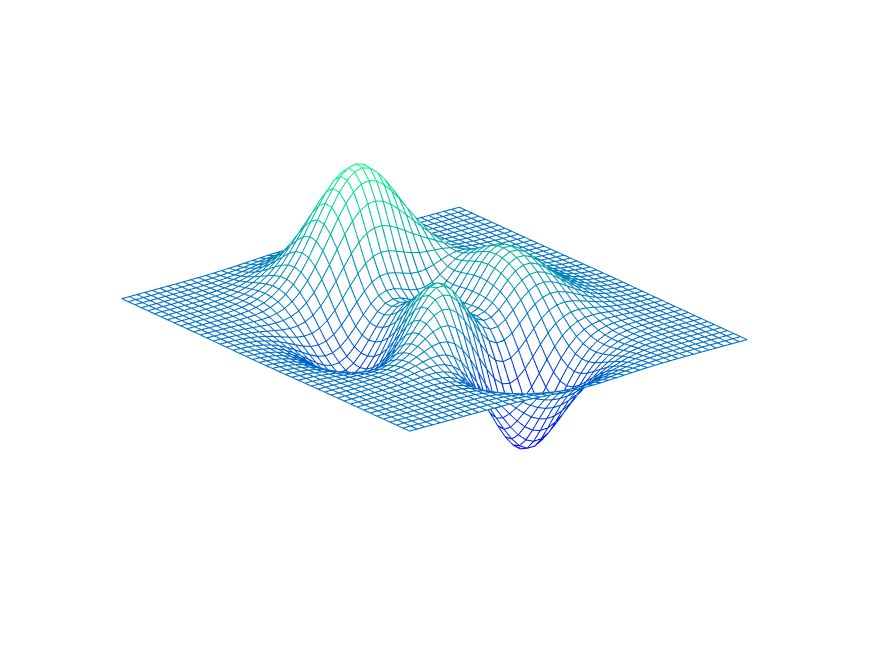
\includegraphics[trim={0cm 0cm 0cm 0cm},clip,height=.2\textheight,width=1\textwidth,keepaspectratio]{../Figures/exfigure1} \\
					\end{center}
					\fignotes{Add standalone description. You can reference sections like \ref{sec:data} and variables like \lastobs.} 
				\end{minipage}
			\end{center}
		\end{figure}
	}
\end{document}
% trim = {<left> <lower> <right> <upper>}


}{}	% Closes \iftoggle{fulldraft}


\section{Section} \label{sec:analysis}
\iftoggle{toclinks}{\gototoc}{} % Turn it on/off in packages.tex, command in macros.tex
\iftoggle{cboxes}{	   				  % Turn it on/off in packages.tex
	\begin{boxeditems}
		\item Task.
	\end{boxeditems}}{}

Section takeaway.

\iftoggle{fulldraft}{					% Turn it on/off in packages.tex
Section content.

}{}	% Closes \iftoggle{fulldraft}

\subsection{Subsection}
\iftoggle{toclinks}{\gototoc}{} % Turn it on/off in packages.tex, command in macros.tex

Subsection takeaway.

\iftoggle{fulldraft}{					% Turn it on/off in packages.tex
Subsection content.

}{}	% Closes \iftoggle{fulldraft}

\subsubsection{Sub-subsection}
Sub-subsection takeaway.

\iftoggle{fulldraft}{					% Turn it on/off in packages.tex
Sub-subsection content.

}{}	% Closes \iftoggle{fulldraft}


\section{Conclusions}\label{sec:conclusions}
\iftoggle{toclinks}{\gototoc}{} % Turn it on/off in packages.tex, command in macros.tex
\iftoggle{cboxes}{	   				 % Turn it on/off in packages.tex
	\begin{boxeditems}
		\item Review. 
	\end{boxeditems}}{}

Summary.

\iftoggle{fulldraft}{					% Turn it on/off in packages.tex
Remarks.

}{}	% Closes \iftoggle{fulldraft}


\iftoggle{fulldraft}{					% Turn it on/off in packages.tex
	\section*{Acknowledgments}
	\protect\linespread{1}\protect\selectfont
We thank \(\langle\)LIST OF NAMES\(\rangle\), and seminar participants at \(\langle\)LIST OF SEMINARS\(\rangle\) for their helpful comments. We also thank \(\langle\)LIST OF NAMES\(\rangle\) for research assistance. The views expressed in this paper are the sole responsibility of the authors and should not be interpreted as reflecting the views of \(\langle\)LIST OF INSTITUTIONS\(\rangle\). All errors are our own. The codes generating the results described in the paper are available at \url{https://website.extension}. Declarations of interest: \(\langle\)LIST\(\rangle\).
% Funding: This work was supported by the Institutes of XXXX [grant numbers xxxx, yyyy]; the XXXX Foundation, Address [grant number zzzz]; and the XXXX Institute of XXXX [grant number aaaa]. Otherwise: This research did not receive any specific grant from funding agencies in the public, commercial, or not-for-profit sectors.
}{}	% Closes \iftoggle{fulldraft}

%---------------------------------------------------------------
% Figures and Tables
%---------------------------------------------------------------

%\newpage
%\input{../Figures/fig1}	% \ref{fig:fig1}
%\input{../Tables/tab1}		% \ref{tab:tab1}